% Options for packages loaded elsewhere
\PassOptionsToPackage{unicode}{hyperref}
\PassOptionsToPackage{hyphens}{url}
%
\documentclass[
  11pt,
  a4paper,
]{article}
\usepackage{amsmath,amssymb}
\usepackage{lmodern}
\usepackage{iftex}
\ifPDFTeX
  \usepackage[T1]{fontenc}
  \usepackage[utf8]{inputenc}
  \usepackage{textcomp} % provide euro and other symbols
\else % if luatex or xetex
  \ifXeTeX
    \usepackage{zxjatype} 
    \usepackage[ipaex]{zxjafont}
    \setromanfont{Times New Roman}
  \fi
  \usepackage{unicode-math}
  \defaultfontfeatures{Scale=MatchLowercase}
  \defaultfontfeatures[\rmfamily]{Ligatures=TeX,Scale=1}
\fi
% Use upquote if available, for straight quotes in verbatim environments
\IfFileExists{upquote.sty}{\usepackage{upquote}}{}
\IfFileExists{microtype.sty}{% use microtype if available
  \usepackage[]{microtype}
  \UseMicrotypeSet[protrusion]{basicmath} % disable protrusion for tt fonts
}{}
\usepackage{xcolor}
\IfFileExists{xurl.sty}{\usepackage{xurl}}{} % add URL line breaks if available
\IfFileExists{bookmark.sty}{\usepackage{bookmark}}{\usepackage{hyperref}}
\hypersetup{
  pdftitle={Appendix ``Estimating Effect of Tax Incentives on Donations Considering Self-Selection of Tax Incentives in South Korea''},
  hidelinks,
  pdfcreator={LaTeX via pandoc}}
\urlstyle{same} % disable monospaced font for URLs
\usepackage[left=3cm,right=3cm,top=3cm,bottom=3cm]{geometry}

\usepackage{setspace}
\renewcommand{\baselinestretch}{1.5}
\usepackage{float}

\usepackage{longtable,booktabs,array}
\usepackage{threeparttable, threeparttablex, multirow}
\usepackage{calc} % for calculating minipage widths
% Correct order of tables after \paragraph or \subparagraph
\usepackage{etoolbox}
\makeatletter
\patchcmd\longtable{\par}{\if@noskipsec\mbox{}\fi\par}{}{}
\makeatother
% Allow footnotes in longtable head/foot
\IfFileExists{footnotehyper.sty}{\usepackage{footnotehyper}}{\usepackage{footnote}}
\makesavenoteenv{longtable}
\usepackage{graphicx}
\makeatletter
\def\maxwidth{\ifdim\Gin@nat@width>\linewidth\linewidth\else\Gin@nat@width\fi}
\def\maxheight{\ifdim\Gin@nat@height>\textheight\textheight\else\Gin@nat@height\fi}
\makeatother
% Scale images if necessary, so that they will not overflow the page
% margins by default, and it is still possible to overwrite the defaults
% using explicit options in \includegraphics[width, height, ...]{}
\setkeys{Gin}{width=\maxwidth,height=\maxheight,keepaspectratio}
% Set default figure placement to htbp
\makeatletter
\def\fps@figure{htbp}
\makeatother
\setlength{\emergencystretch}{3em} % prevent overfull lines
\providecommand{\tightlist}{%
  \setlength{\itemsep}{0pt}\setlength{\parskip}{0pt}}
\setcounter{secnumdepth}{5}


\ifLuaTeX
  \usepackage{selnolig}  % disable illegal ligatures
\fi

\makeatletter
\def\@fnsymbol#1{\ensuremath{\ifcase#1\or \dagger\or \ddagger\or
   \mathsection\or \mathparagraph\or \|\or **\or \dagger\dagger
   \or \ddagger\ddagger \else\@ctrerr\fi}}
    \makeatother
\title{Appendix
``Estimating Effect of Tax Incentives on Donations Considering Self-Selection of Tax Incentives in South Korea''  }
\author{
    Hiroki Kato
  \thanks{Graduate School of Economics, Osaka University, Japan. E-mail: vge008kh@stundent.econ.osaka-u.ac.jp  }
  \and
    Tsuyoshi Goto
  \thanks{Graduate School of Social Sciences, Chiba University, Japan. E-mail: t.goto@chiba-u.jp  }
  \and
    Youngrok Kim
  \thanks{Graduate School of Economics, Kobe University, Japan.  }
  \and
  }

\date{2022/04/18}


\begin{document}
\begin{spacing}{1}
  \maketitle
\end{spacing}

{
\setcounter{tocdepth}{2}
\tableofcontents
}
\hypertarget{appendix-appendix}{%
\appendix}


\hypertarget{addtab}{%
\section{Additional Tables and Figures}\label{addtab}}

\begin{figure}[t]

{\centering 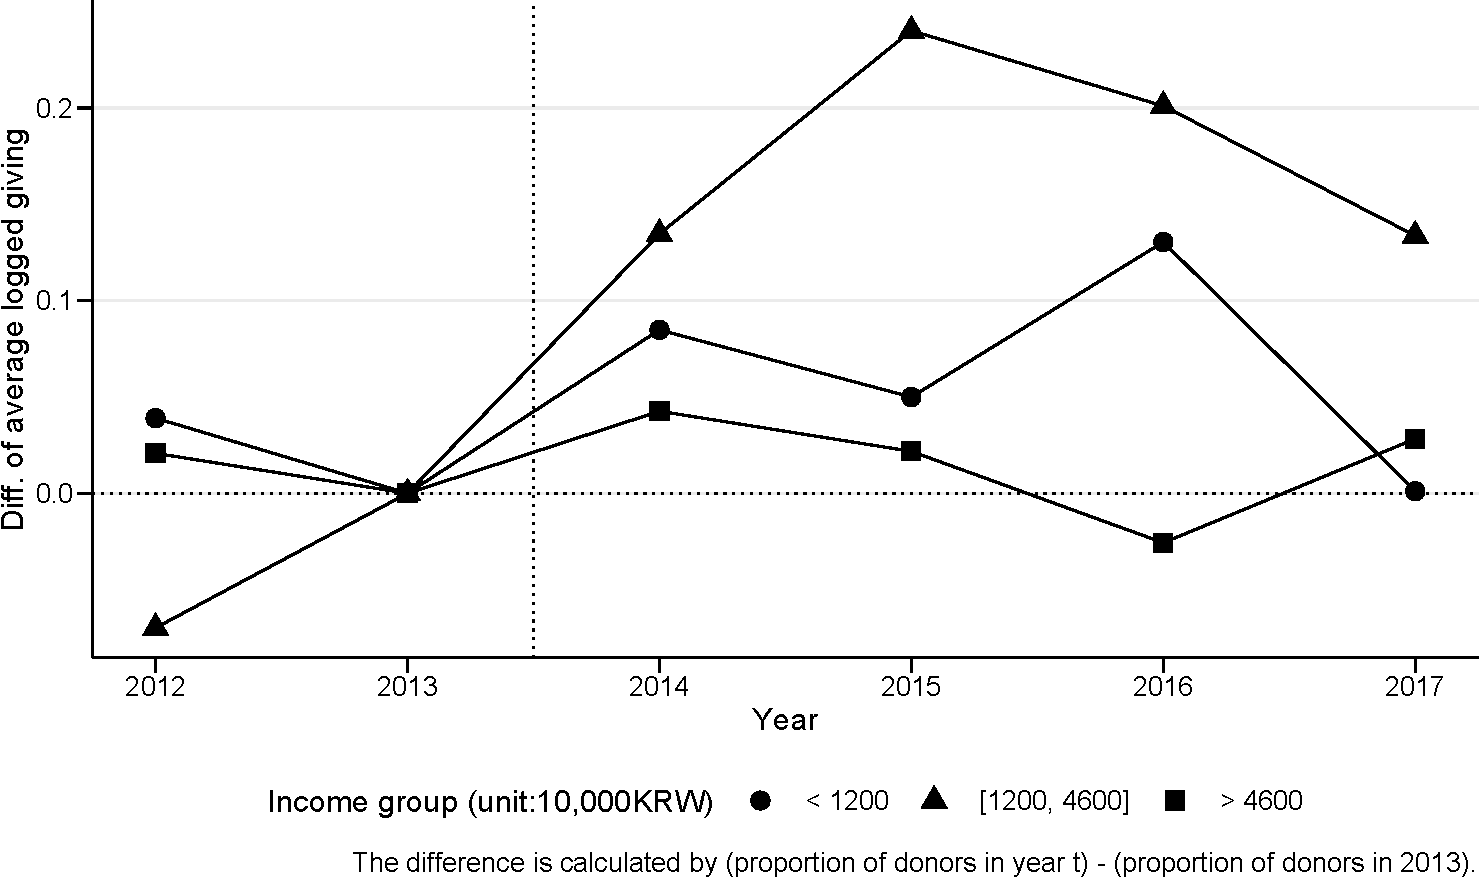
\includegraphics{C:/Users/vge00/Desktop/NaSTaB/docs/paper/appendix_files/figure-latex/SummaryGivingIntensive-1} 

}

\caption{Average Logged Giving by Three Income Groups Conditional on Donors. Notes: We created three income groups, with the relative price of giving rising (circle), unchanged (triangle), and falling (square) between 2013 and 2014. The group averages are normalized to be zero in 2013.}\label{fig:SummaryGivingIntensive}
\end{figure}
\begin{figure}[t]

{\centering 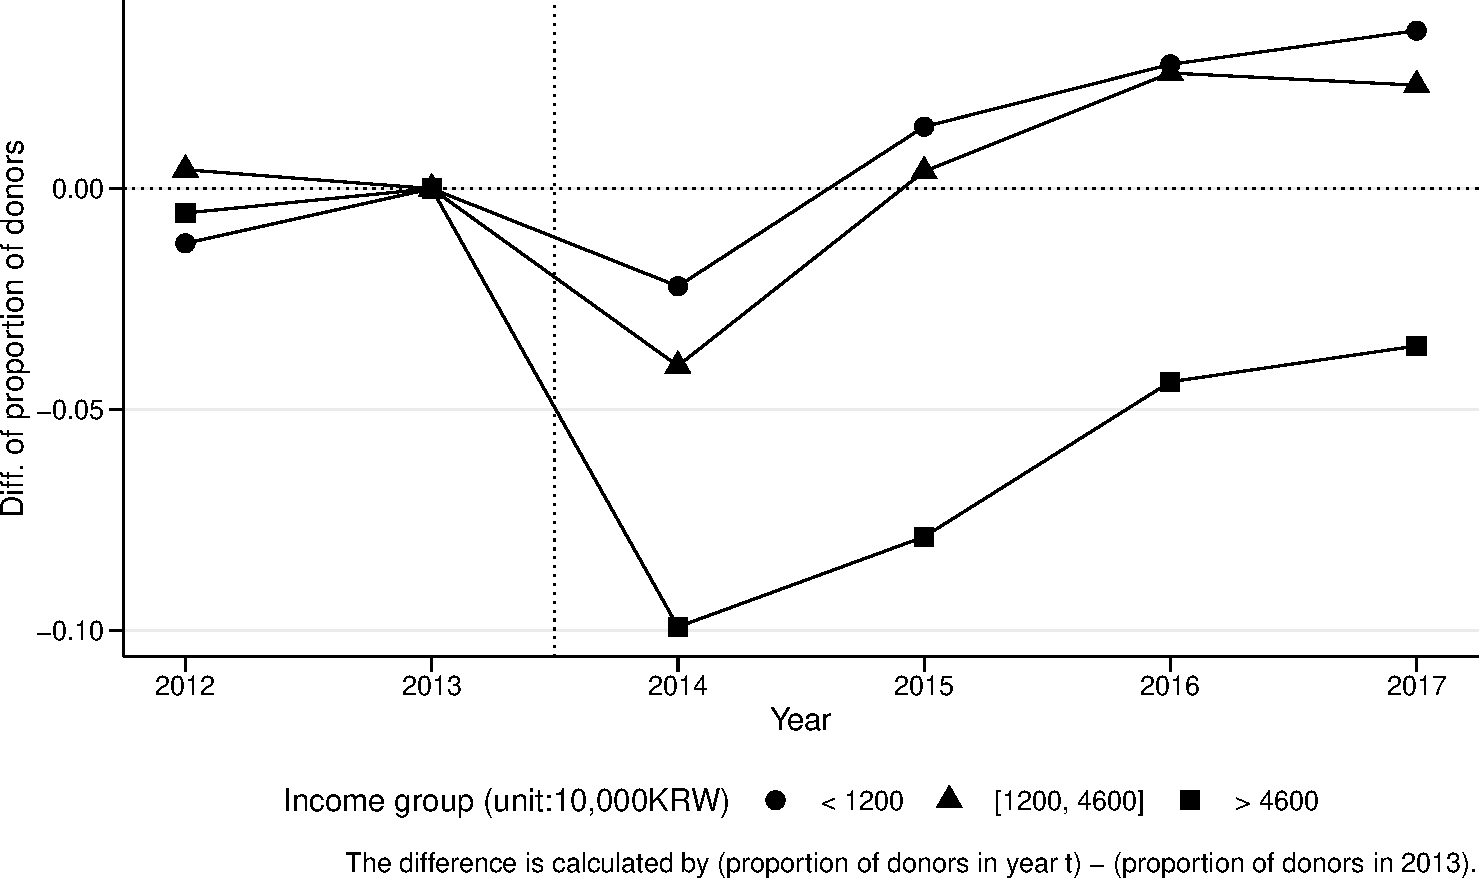
\includegraphics{C:/Users/vge00/Desktop/NaSTaB/docs/paper/appendix_files/figure-latex/SummaryGivingExtensive-1} 

}

\caption{Proportion of Donors by Three Income Groups. Notes: We created three income groups, with the relative price of giving rising (circle), unchanged (triangle), and falling (square) between 2013 and 2014. The group averages are normalized to be zero in 2013.}\label{fig:SummaryGivingExtensive}
\end{figure}

\begin{figure}[t]

{\centering 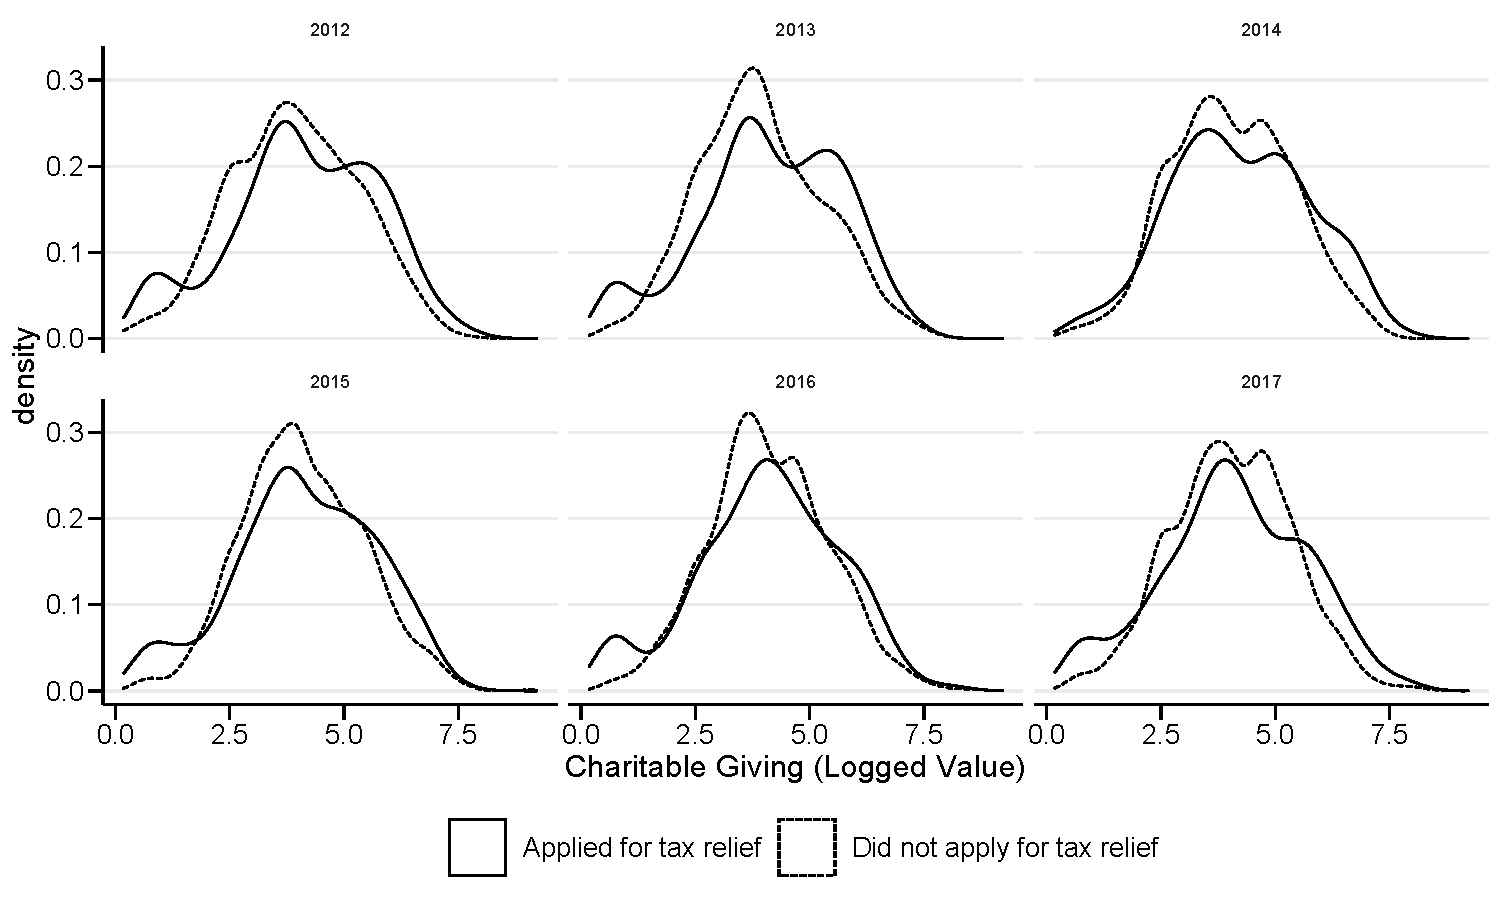
\includegraphics{C:/Users/vge00/Desktop/NaSTaB/docs/paper/appendix_files/figure-latex/SummaryGivingIntensiveDist-1} 

}

\caption{Estimated Distribution of Charitable Giving among Donors in Each Year}\label{fig:SummaryGivingIntensiveDist}
\end{figure}

\begin{figure}[t]

{\centering 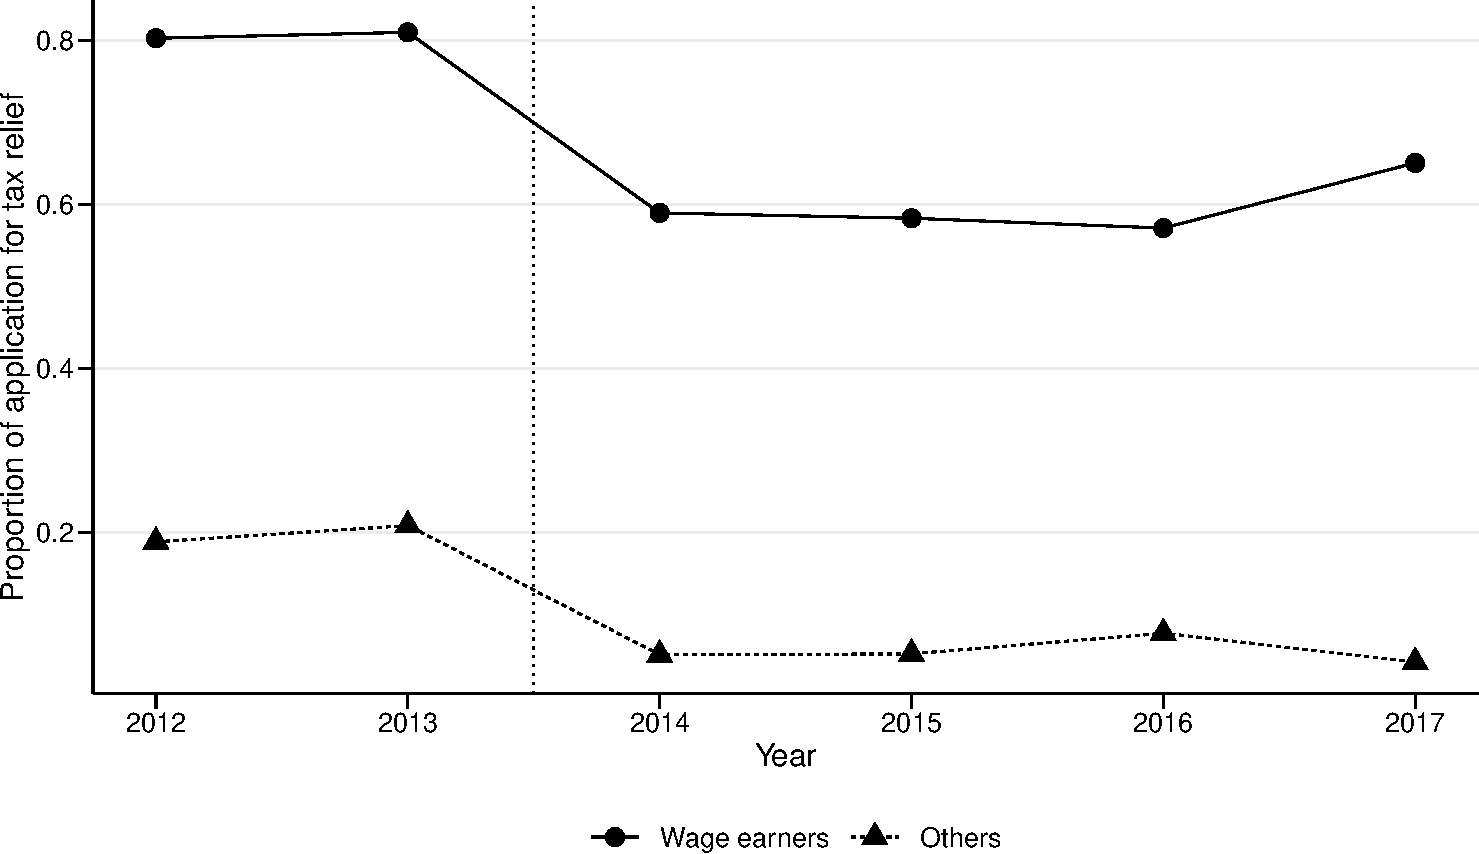
\includegraphics{C:/Users/vge00/Desktop/NaSTaB/docs/paper/appendix_files/figure-latex/SummaryReliefbyEarner2-1} 

}

\caption{Share of Tax Relief by Wage Earners Conditional on Donors. Notes: A solid line is the share of applying for tax relief among wage eaners. A dashed line is the share of applying for tax relief other than wage earners.}\label{fig:SummaryReliefbyEarner2}
\end{figure}

\end{document}
